%% Appendix of the extended (arXiv) version of main_camera_ready_9p.tex.
%% Included only when \arxivtrue is set in the main file. Every number below is
%% re-derived by scripts/analyze_cameraready_e10_e7.py, analyze_cameraready_e6_e12.py,
%% and analyze_cameraready_topk_reruns.py (no model calls); the code guide is
%% docs/2026-10-15_cameraready_experiments_guide.md.

%% Long texttt names and inline math cannot hyphenate; let the appendix stretch spaces instead.
\sloppy
\section{Staged controls}\label{app:staged}
\paragraph{Construction.}
Both controls start from R-PAL$^{+}$ and change one thing at a time (Table~\ref{tab:app-staged-build}). Staged R-PAL$^{+}$ (Staged) keeps the inputs of R-PAL$^{+}$, that is, the same top-4 retrieval, the same reference rendering, and the same taxonomy text, verbatim. It splits the single call of R-PAL$^{+}$ into the five VerifiQuant stages, one model call each. Every stage receives the taxonomy, a fixed frame that names the five stages and the current one, the question, the context, and a JSON answer format, and the first stage that does not pass ends the case. The program stage writes \texttt{solve()}, which runs in the sandbox of R-PAL$^{+}$. Every check is a model judgment. Spec-prompted R-PAL$^{+}$ (Staged+Spec) keeps the same stages and adds, as text only, the contract content that the matching VerifiQuant gate uses. Neither control executes a contract. The prompts are printed in full in Appendix~\ref{app:prompts}.

\begin{table*}[t]
\caption{What each stage of the two staged controls receives.}
\label{tab:app-staged-build}
\small
\begin{tabular}{@{}l>{\raggedright\arraybackslash}p{0.14\textwidth}>{\raggedright\arraybackslash}p{0.30\textwidth}>{\raggedright\arraybackslash}p{0.36\textwidth}@{}}
\toprule
Stage & Decides & Staged receives & Staged+Spec also receives \\
\midrule
1 Scope & M or N, and picks a candidate & the top-4 reference functions (title, summary, code) & each candidate's selection hints, applicable and non-applicable conditions, and scope boundaries \\
2 Inputs & F, and binds each input & the chosen reference function & the contract's input schema (name, type, required, unit, description) \\
3 Boundaries & E & the chosen function and the bound inputs & the contract's declared boundary checks (rule, description, expression), to be judged, not run \\
4 Ambiguity & I\textsubscript{HARD} or I\textsubscript{SOFT} & the chosen function and the bound inputs & the contract's declared semantic hints (trigger, options, level, default assumption) \\
5 Program & writes \texttt{solve()} & the chosen function, the bound inputs, and any I\textsubscript{SOFT} assumption & nothing further \\
\bottomrule
\end{tabular}
\end{table*}

\paragraph{Results.}
Table~\ref{tab:app-staged} places both controls between R-PAL$^{+}$ and VerifiQuant on Gemini 2.5 Flash, and each row differs from the one above in a single respect. Trap columns, and the clean columns of Staged and Staged+Spec, are means of three runs. Sel is accuracy among the clean questions a system answers. All four are precise when they answer and differ in how often they answer.

\begin{table*}[t]
\caption{Staged controls on the 80 traps and the 250 clean questions.}
\label{tab:app-staged}
\small
\begin{tabular}{@{}llrrrrrrrrrr@{}}
\toprule
& & \multicolumn{7}{c}{Traps (80)} & \multicolumn{3}{c}{Clean (250)} \\
\cmidrule(lr){3-9}\cmidrule(l){10-12}
System & Differs from the row above by & FNAR & F & E & I & N & Diag & Act & Cov & Acc & Sel \\
\midrule
R-PAL$^{+}$ & --- & 27.5\% & 0\% & 30.0\% & 80.0\% & 0\% & 65.4\% & 55.8\% & 92.9\% & 92.0\% & 99.0\% \\
Staged & five separate stage calls & 15.8\% & 0\% & 20.0\% & 43.3\% & 0\% & 73.8\% & 69.6\% & \stagedOneCov{} & \stagedOneAcc{} & 99.4\% \\
Staged+Spec & contract content as text & 8.8\% & 0\% & 0\% & 35.0\% & 0\% & 82.1\% & 80.0\% & \stagedTwoCov{} & \stagedTwoAcc{} & 98.4\% \\
VerifiQuant & checks executed as code & 10.4\% & 10.0\% & 8.3\% & 21.7\% & 1.7\% & 76.7\% & 75.4\% & 84.0\% & 81.2\% & 96.7\% \\
\bottomrule
\end{tabular}
\end{table*}

Step by step, with 95\% intervals from the base-question-clustered bootstrap of \S\ref{sec:v2res}, staging lowers trap FNAR by 11.7 points $[5.5, 18.6]$, declared contract content by a further 7.1 points $[1.7, 13.1]$, and execution changes it by $-1.7$ points $[-8.3, 4.8]$. On the clean questions Staged covers \stagedOneCov{} and Staged+Spec \stagedTwoCov{} (means of three runs), against $84.0\%$ for VerifiQuant. VerifiQuant answers more clean questions than Staged+Spec in every run (exact McNemar $p<.01$ for coverage and $p<.03$ for accuracy in each run). Staged+Spec leaves about 23 more questions unanswered than VerifiQuant, and a mean of 16.3 per run are programs the model wrote that fail to run, so most of the coverage gap comes from executing model-written code rather than from gate decisions.

\paragraph{Price of the reduction.}
Read against R-PAL$^{+}$, each point of trap FNAR removed costs Staged $2.2$ points of clean accuracy, Staged+Spec $1.0$ point, and VerifiQuant $0.6$ point. These are the slopes from R-PAL$^{+}$ to each system on a plane of clean accuracy against trap FNAR, so they do not depend on the size of either set. In questions, Staged answers a mean of $63.3$ fewer clean questions correctly for $9.3$ fewer trap acceptances, Staged+Spec $46.0$ for $15.0$, and VerifiQuant $27$ for $13.7$, that is, $6.8$, $3.1$, and $2.0$ correct clean answers per trap acceptance avoided. This second form scales with the ratio of the two set sizes (250 to 80), which is why the body keeps the two axes separate. On these point estimates VerifiQuant pays the least per point removed. Its clean figure comes from one run, and the others are means of three runs.

Three disclosures apply. First, each stage uses one prompt wording, and after a five-trap smoke test we changed one phrase, ``exactly one candidate'', which the model had read literally and answered N whenever several candidates fit. Second, a program that fails to run counts as no number, as in R-PAL$^{+}$. This happened on three Staged and two Staged+Spec trap cases, all of type I, and counting them as acceptances would raise trap FNAR to 17.1\% and 9.6\%. Third, the controls were run after the main experiments, on the same backbone, retrieval, and scoring.

\section{Scripted user}\label{app:scripted}
The 26 traps that remove a required input (20 F) or a hard convention (6 I\textsubscript{HARD}) are the ones on which asking the user is the correct response. The first turn is the existing output: the three depth-4 VerifiQuant runs and the three R-PAL$^{+}$ runs. When a system withholds a number, a scripted user replies once and the system runs again with the reply appended to the context. The user involves no model and never sees the gold answer. For an F trap it restates the exact span the trap replaced with a placeholder, with its unit, as in ``The tax liability is \$12,000.''. For an I\textsubscript{HARD} trap it fills one fixed template per ambiguity family, such as ``It is a call option.'' or ``Use the FIFO method.''. The strict user replies only when the first turn named the removed field or convention, matching field names with underscores and spaces treated alike and conventions as whole words. The lenient user replies to every abstention. Table~\ref{tab:app-scripted} gives the counts per run, three runs per system.

\begin{table}[t]
\caption{Scripted user on the 26 incomplete traps.}
\label{tab:app-scripted}
\small
\begin{tabular}{@{}lrr@{}}
\toprule
& VerifiQuant & R-PAL$^{+}$ \\
\midrule
Number at turn 1 & 3 / 3 / 4 & 3 / 3 / 3 \\
Withheld and named the item & 22 / 21 / 20 & 18 / 19 / 20 \\
Correct after reply, strict & 20 / 19 / 18 & 18 / 17 / 19 \\
Correct after reply, lenient & 20 / 19 / 18 & 22 / 20 / 21 \\
Wrong number after reply & 0 & 0 \\
\addlinespace
Strict, F only (of 20) & 16 / 16 / 16 & 16 / 15 / 17 \\
Strict, I\textsubscript{HARD} only (of 6) & 4 / 3 / 2 & 2 / 2 / 2 \\
\bottomrule
\end{tabular}
\end{table}

Strict recovery is $73.1\%$ for VerifiQuant and $69.2\%$ for R-PAL$^{+}$, a difference of $+3.8$ points with a 95\% interval of $[-16.7, 24.4]$ over 26 clustered traps. VerifiQuant asks the right question more often only on the six I\textsubscript{HARD} traps, too few to support a claim. The lenient user lifts R-PAL$^{+}$ to $80.8\%$ because it names fields in prose, such as ``back-end ratio'' for \texttt{back\_end\_limit}, which the literal match misses. VerifiQuant's two F traps answered at turn 1 are the declared-default case of \S\ref{sec:v2rq2}, and its unrecovered cases either picked a contract that asks for a different field, raised a new convention question after the reply, or stopped at F after the convention was supplied. The reply template is fixed and a single sentence, so these figures bound what a cooperative but terse user recovers rather than what a real user would.

\section{A second backbone}\label{app:pro}
Table~\ref{tab:app-pro} repeats the trap comparison of \S\ref{sec:v2rq2} with Gemini 2.5 Pro for every model call, three runs per system, next to the Flash figures of Table~\ref{tab:v2main}.

\begin{table}[t]
\caption{Trap results with Gemini 2.5 Pro.}
\label{tab:app-pro}
\small
\begin{tabular}{@{}lrrrr@{}}
\toprule
& \multicolumn{2}{c}{R-PAL$^{+}$} & \multicolumn{2}{c}{VerifiQuant} \\
\cmidrule(lr){2-3}\cmidrule(l){4-5}
& Flash & Pro & Flash & Pro \\
\midrule
FNAR (mean) & 27.5\% & 22.1\% & 10.4\% & 10.4\% \\
E & 30.0\% & 20.0\% & 8.3\% & 13.3\% \\
I & 80.0\% & 68.3\% & 21.7\% & 13.3\% \\
F / N & 0 / 0\% & 0 / 0\% & 10.0 / 1.7\% & 10.0 / 5.0\% \\
Diag / Act & 65.4 / 55.8\% & 66.7 / 42.5\% & 76.7 / 75.4\% & 75.0 / 73.8\% \\
\bottomrule
\end{tabular}
\end{table}

The gap is 11.7 points on Pro, with a 95\% interval of $[1.7, 21.5]$, against 17.1 points on Flash. Per run, Pro gives R-PAL$^{+}$ 25.0, 21.25, and 20.0\% and VerifiQuant 12.5, 8.75, and 10.0\%. Pro improves R-PAL$^{+}$ on E and I and leaves VerifiQuant unchanged, and the remaining gap lies almost entirely in I. Pro belongs to the same model family as Flash, and we ran only the traps on it, so it places no point on the safety--utility plane.

\section{Run-level results and retrieval depth}\label{app:reruns}
The paired tests of \S\ref{sec:v2res} use per-question binary outcomes from one audited R-PAL run on all clean questions and the canonical VerifiQuant $K{=}3$ run on the same case IDs, not averages over repeats.
The submitted version reported one VerifiQuant trap run, made at retrieval depth 3 because the runner's default was 3, while the protocol and R-PAL$^{+}$ used 4. The same default affected the out-of-library split, the gate ablation, and the library sweep. All four were rerun at depth 4 with the same questions, libraries, and scoring, and the body reports the reruns. No conclusion changes. Table~\ref{tab:app-trapruns} lists trap FNAR run by run, with depth the number of retrieved candidates, and Table~\ref{tab:app-depth} compares the other three evaluations at both depths.

\begin{table}[t]
\caption{Trap FNAR by run.}
\label{tab:app-trapruns}
\small
\begin{tabular}{@{}llr@{}}
\toprule
System & Depth & FNAR per run \\
\midrule
VerifiQuant (submitted) & 3 & 11.25\% \\
VerifiQuant (rerun) & 3 & 7.5\% \\
VerifiQuant (reported) & 4 & 12.5 / 10.0 / 8.75\% \\
R-PAL$^{+}$ (reported) & 4 & 26.25 / 30.0 / 26.25\% \\
R-PAL$^{+}$ (drift check) & 4 & 26.25\% \\
\bottomrule
\end{tabular}
\end{table}

Across five VerifiQuant runs and four R-PAL$^{+}$ runs the ranges do not overlap, and the later R-PAL$^{+}$ run falls inside its earlier range, so the backbone did not drift between July and October. Two identical VerifiQuant runs disagree on the diagnosis of 10 of the 80 traps because selection, binding, and ambiguity checks are model calls. A single run should therefore not be compared with a mean.

\begin{table}[t]
\caption{Depth 3 against depth 4.}
\label{tab:app-depth}
\small
\setlength{\tabcolsep}{4pt}
\begin{tabular}{@{}lrr@{}}
\toprule
Quantity & Depth 3 & Depth 4 \\
\midrule
OOD abstain / correct / SWR & 88.9 / 7.0 / 4.0\% & 88.9 / 7.0 / 4.0\% \\
OOD selective accuracy / ID abstain & 63.6 / 19.6\% & 63.6 / 19.6\% \\
Gate ablation, compute only & 87.6\% / 6.4\% / 15 & 90.0\% / 5.6\% / 11 \\
Gate ablation, + F/E & 86.8\% / 4.4\% / 22 & 87.2\% / 5.6\% / 18 \\
Gate ablation, + I & 79.6\% / 4.4\% / 40 & 82.4\% / 4.8\% / 32 \\
Gate ablation, full funnel & 79.2\% / 4.0\% / 42 & 82.0\% / 4.4\% / 34 \\
Sweep, ID accuracy range & 81.6--84.0\% & 83.2--87.1\% \\
Sweep, OOD abstain (10\%$\to$75\%) & 91.6$\to$80.6\% & 91.1$\to$79.0\% \\
Sweep, OOD SWR (10\%$\to$75\%) & 1.3$\to$4.8\% & 2.2$\to$4.8\% \\
\bottomrule
\end{tabular}
\end{table}

The out-of-library aggregates are identical, although 10 of the 250 verdicts changed in offsetting directions. Gate-ablation rows read accuracy, SWR, and abstentions. The latency figures of \S\ref{sec:v2res} come from the earlier sequential depth-3 ladder, because the depth-4 rerun executed its rungs concurrently. They are wall-clock means that include provider-side variance and retries, and we do not report token accounting.

\paragraph{F-trap construction check.}
The F operator removes an input the contract requires. Checking every F trap against that rule, through the contract's \texttt{required} flag and any default in the contract or its reference function, finds 3 of the 20 that fail it. Two (F-test-1263 and F-test-1559) remove a share count that the contract marks optional with a default of 100 shares, one option contract, which the public reference function also declares. Answering with the default is correct, so these two traps are mislabeled. VerifiQuant answers both correctly in every run and is scored as accepting them. The third (F-test-1271) removes a unit count that the contract marks optional with a placeholder default of 0, although the question cannot be answered without it. Its label is right and the contract is underspecified, and VerifiQuant requests the field in every run.
All three come from one generator step. It drew F candidates from every argument of the reference function's signature, including arguments with defaults, instead of from the inputs the contract marks required. The two mislabeled traps therefore penalize exactly the behavior a declared default licenses: VerifiQuant applies the default and is scored as accepting, while the systems that decline both, R-PAL$^{+}$ and the two staged controls, are scored as correct. R-PAL answers F-test-1263 correctly as well. Across the 250 cards, 34 of the 38 optional or defaulted inputs take their default from the reference function's signature, 4 state no default, and none takes a value that appears only in the source question. Six have a placeholder default (0, None, or False). Three are genuine optional values (the \texttt{refundable} and \texttt{annualize} switches and a zero dividend), and three, the unit count of the third case, a purchase price, and an exchange rate, may be required whenever the formula's branch uses them. A future trap set should draw F candidates only from inputs the contract marks required and that no default covers, and the contract builder should mark such branch-dependent inputs as conditionally required. We keep the released 80 traps for comparability with the submitted version and report the sensitivity below. Table~\ref{tab:app-fsens} rescores every system without the failing traps, with the scorer and bootstrap of \S\ref{sec:v2res}.

\begin{table}[t]
\caption{Trap FNAR without the F traps that fail the construction check.}
\label{tab:app-fsens}
\small
\setlength{\tabcolsep}{3pt}
\begin{tabular}{@{}lrrrr@{}}
\toprule
Trap set & VQ & R-PAL$^{+}$ & Gap [95\% CI] & S+S$-$VQ \\
\midrule
All 80 traps (80) & 10.4\% & 27.5\% & $17.1$ $[6.8, 27.0]$ & $-1.7$ \\
Without the 2 mislabeled (78) & 8.1\% & 28.2\% & $20.1$ $[11.0, 29.2]$ & $+0.9$ \\
Without all 3 failing (77) & 8.2\% & 28.6\% & $20.3$ $[11.1, 29.5]$ & $+0.9$ \\
\bottomrule
\end{tabular}
\end{table}

Columns give the 3-run mean FNAR, the R-PAL$^{+}$ minus VerifiQuant gap in points, and the Staged+Spec minus VerifiQuant difference in points. Without the mislabeled traps VerifiQuant's F rate is $0\%$, the gap widens, and Staged+Spec remains level with VerifiQuant.

\paragraph{Why depth 4.} On the 250 clean questions, where each question's gold contract is in the library by construction, the gold card is retrieved at rank 1 in the median case and appears in the top 4 for $94.8\%$ of questions. Widening to 8 adds $2.4$ points, and widening to 16 adds $4.0$. A larger $k$ or a stronger retriever therefore has under five points of headroom on in-library queries, which is why we hold $k{=}4$ fixed rather than tuning it.

\section{Human-labeled set: construction, labels, and scoring}\label{app:human}
This appendix gives the full protocol behind \S\ref{sec:v2ext} and \S\ref{sec:v2rq4}.

\paragraph{Construction and annotation.}
The F/E/I/N traps are contract-derived, so a skeptic can ask whether their labels merely re-encode our own checks (\S\ref{sec:v2design}). We therefore need queries whose correct handling is decided by people who see neither our contracts nor our systems.
To test the governance boundary against labels defined \emph{independently} of our contracts, we build a second evaluation whose ground truth comes from human domain experts with no access to any system, contract, or gold answer. GPT-5.2 authored the 80 naturalistic queries from FinanceReasoning topics with no access to our contracts, the M/N/F/E/I/C taxonomy, gold answers, or any system output. An audit before labeling found that all 18 queries of the missing-input stratum had left the context empty, so the stratum could be recognized at a glance and no single input was actually missing. We revised these 18 offline with an OpenAI Codex agent, seeded by the GPT-5.2 versions, because a further call to the external author was not yet cleared for data egress. Each revision keeps its source topic and persona, gives two to five labeled figures, omits exactly one indispensable numeric input, avoids any word that marks the omission, and adds no convention ambiguity. An automatic check confirmed these properties for all 18, a person read every revision, and the other 62 queries are unchanged. The revision ran inside our repository, so unlike the 62 it is not blind to our contracts. The provenance file records the 18 as \texttt{gpt-5.2\_seed\_then\_codex\_curated\_v3}. Both authors differ from the solver stack (Gemini 2.5 Flash, used by every evaluated system), so a question's messiness is uncorrelated with what any solver finds easy. Every label was collected after the revision.
The source questions come from FinanceReasoning items outside the 250 of \S\ref{sec:v2design}. Rewriting the 250 themselves would guarantee a contract for every item and turn the test into one of paraphrase robustness inside the library. Drawing elsewhere keeps the labels independent of our contracts, at the cost that the set is \emph{library-agnostic}: it mixes in-library and out-of-library questions in a proportion we do not set.
Items are drawn from four latent conditions, well-posed (27), missing a required input (18), ambiguous in a material convention (18), and judgment or out-of-scope (17). An unstratified first draft was skewed toward answerable queries and left too few non-answer items to estimate an acceptance rate, which is why we stratify by user intent. The condition is a sampling stratification, never a label, and is hidden from annotators, so the panel's label distribution need not match it. Five finance-trained annotators, blind to the source question, the generating condition, and every system output, independently assign one of four actions with a one-sentence rationale. Majority labels are frozen before any system is scored, all 80 items reach a first-pass majority so no adjudication was needed, and we report Fleiss' $\kappa$ as reliability. Full curation checks, instructions, and worked examples ship with the released audit trail.

\paragraph{Label definitions.}
Annotators assign one of four labels per item by a top-down rule, stopping at the first ``yes'': is the ask itself not ``compute one number'' (advice, a forecast, or a request needing unavailable data)? then \textsc{out-of-scope}. Is a required numeric value missing from the text? then \textsc{request-info}. Are all values present, but would an interpretation choice (percent vs.\ decimal, which period, which metric, day-count basis, gross vs.\ net, per-share vs.\ total) change the number? then \textsc{clarify}. Otherwise, a complete and unambiguous computation is \textsc{answer}.
The \textsc{request-info} versus \textsc{clarify} contrast (a missing number versus an unclear interpretation) is trained explicitly, and the full instructions ship with the audit trail.
Each action maps onto a funnel outcome (\textsc{answer}$\leftrightarrow$compute, \textsc{request-info}$\leftrightarrow$F, \textsc{clarify}$\leftrightarrow$I, \textsc{out-of-scope}$\leftrightarrow$N/M), so emitting a confident number where the human label is \textsc{request-info}, \textsc{clarify}, or \textsc{out-of-scope} is a false numeric acceptance defined by human judgment rather than by our taxonomy.

\paragraph{Scoring protocol.}
Each system's raw output is normalized to an action in $\{$A, R, C, O$\}$, with the full per-system mapping in the released audit trail. Two conventions matter for reading Table~\ref{tab:v2ext}. CoT and plain R-PAL expose only whether they answered, never why they declined, so scoring them four-way would discard credit for correct abstention. Their Match is therefore the binary agreement between answering and a human \textsc{answer} label, whereas R-PAL$^{+}$ and VerifiQuant expose a real R/C/O decision and are scored four-way. An M-refusal is scored \textsc{out-of-scope} per \S\ref{sec:v2ext}, even though every M-refusal here carries an explicit clarification question, which is a conservative reading of our own convention rather than one chosen after seeing the scores: an \textsc{M}$\to$\textsc{clarify} reading would raise VerifiQuant's Match from $32.5\%$ to $35.0\%$. Let $\mathrm{GT}(i)$ be the human majority label of item $i$ over the $n{=}80$ items, $e_S(i){:=}\mathrm{emit}_S(i){\in}\{0,1\}$ whether system $S$ commits a numeric answer on item $i$, and $\mathrm{RCO}=\{i : \mathrm{GT}(i)\neq\text{A}\}$ the $46$ items a plain number is inappropriate for.
\[
\mathrm{HumanFNAR}(S) = \frac{|\{\, i \in \mathrm{RCO} : e_S(i){=}1 \,\}|}{|\mathrm{RCO}|}
\]
A number that carries an I\textsubscript{SOFT} warning counts as emitted. A \textsc{clarify} label means the panel wanted the question asked before any computation, and a warned number does not ask, so this convention is stricter than the trap metric of \S\ref{sec:v2problem}. Human-FNAR is the headline because it needs only whether a number was emitted, which every system exposes, and no gold answer.
Every system answers the same 46 non-\textsc{answer} items, so the tests of \S\ref{sec:v2rq4} are paired. Against plain R-PAL, VerifiQuant alone emits a number on 0 items and R-PAL alone on 22 (exact McNemar $p<10^{-6}$). Against R-PAL$^{+}$ the counts are 3 and 5 ($p{=}.73$), and against CoT 1 and 7 ($p{=}.07$). An unpaired Fisher test on the same rates gives the same reading ($p<10^{-5}$ and $p{=}.74$).
Answer coverage is $\mathrm{AnsCov}(S)=\frac{1}{|\mathrm{AA}|}\sum_{i\in\mathrm{AA}} e_S(i)$ over the 34 items $\mathrm{AA}=\{i:\mathrm{GT}(i)=\text{A}\}$, and Match is the share of the 80 items on which a system's action equals $\mathrm{GT}(i)$, four-way or binary as above. Table~\ref{tab:v2ext} omits accuracy because source gold answers do not transfer after rewriting. Fresh golds constructed for the 34 answerable items serve only the diagnostic analysis above.

\paragraph{What the human set tests.}
Table~\ref{tab:app-human-exits} splits each system's handling by the panel's label. Most items VerifiQuant declines stop at N, so the low Human-FNAR of \S\ref{sec:v2rq4} comes mainly from the library boundary. Where VerifiQuant does select a contract, it asks for the missing input on 5 of 7 \textsc{request-info} items, while R-PAL$^{+}$ asks on all 7 and on 16 of the 20 overall. On the 10 \textsc{clarify} items VerifiQuant raises no hard clarification and asks three questions through M, while R-PAL$^{+}$ raises one. The set therefore supports the scope signal, not a claim that the input and ambiguity checks outperform a single prompt on natural phrasing. The scope signal is also a claim that can be wrong. Of the 24 \textsc{answer} items that stop at N, 7 have an applicable contract that retrieval ranked outside the top 4 (\S\ref{sec:v2rq4}).

\begin{table}[t]
\caption{Handling by human label on the 80 human-labeled queries.}
\label{tab:app-human-exits}
\small
\setlength{\tabcolsep}{3.2pt}
\begin{tabular}{@{}lrrrrrrr@{}}
\toprule
Label (items) & N & M & F & E & I\textsubscript{H} & Num & Other \\
\midrule
\multicolumn{8}{@{}l}{\emph{VerifiQuant}} \\
\textsc{answer} (34) & 24 & 1 & 1 & 1 & 0 & 7 & 0 \\
\textsc{request-info} (20) & 13 & 1 & 5 & 0 & 0 & 1 & 0 \\
\textsc{clarify} (10) & 4 & 3 & 1 & 0 & 0 & 2 & 0 \\
\textsc{out-of-scope} (16) & 11 & 1 & 1 & 2 & 0 & 1 & 0 \\
\midrule
\multicolumn{8}{@{}l}{\emph{R-PAL$^{+}$}} \\
\textsc{answer} (34) & 9 & 0 & 0 & 0 & 0 & 22 & 3 \\
\textsc{request-info} (20) & 4 & 0 & 16 & 0 & 0 & 0 & 0 \\
\textsc{clarify} (10) & 3 & 2 & 0 & 0 & 1 & 4 & 0 \\
\textsc{out-of-scope} (16) & 11 & 0 & 1 & 0 & 1 & 2 & 1 \\
\bottomrule
\end{tabular}
\end{table}

Num counts emitted numbers, including those with an I\textsubscript{SOFT} warning, and Other counts R-PAL$^{+}$ decisions with no number and no gate label, such as a program that failed to run.

\paragraph{Ethical considerations.}
The items are synthetic and contain no personal information, and only labels and rationales about each question were collected. Participation was voluntary, annotators are anonymized as \textit{Annotator}~1--5, and consultation with our institution determined that ethics-committee review was not required.

\paragraph{Released artifacts.}
We release the 250-card contract library, the staged prompts that build it, and the 80-trap set in the repository of \S\ref{sec:v2method}. The human evaluation ships with its 80 queries and provenance, the five per-annotator label files, the frozen majority ground truth, and the agreement report. Scoring and aggregation scripts come with an audit trail that records the scoring conventions and when labels were frozen relative to each system run.


\section{Bounded-repair verifier}\label{app:repair}
Table~\ref{tab:repairbench} breaks the 906 mutants of \S\ref{sec:v2method} down by mutation class. Gen.\ counts generated mutants, Eq.\ the arithmetically equivalent ones that are excluded, Rej./non-eq.\ the rejected share of the rest, and FA the false accepts. The 20 false accepts concentrate in conditional transforms whose guard branch the five sampled bindings did not exercise, including 10 identity mutants.

\begin{table}[t]
\caption{Bounded-repair verifier by mutation class.}
\label{tab:repairbench}
\centering
\begin{tabular}{@{}lrrrr@{}}
\toprule
Mutation class & Gen. & Eq. & Rej./non-eq. & FA \\
\midrule
function-call injection & 179 & 0 & 179/179 (100\%) & 0 \\
oversized AST & 179 & 0 & 179/179 (100\%) & 0 \\
operator swap & 171 & 8 & 159/163 (97.5\%) & 4 \\
coefficient perturbation & 164 & 9 & 152/155 (98.1\%) & 3 \\
variable swap & 34 & 2 & 29/32 (90.6\%) & 3 \\
identity (no-op) & 179 & 8 & 161/171 (94.2\%) & 10 \\
\midrule
Total & 906 & 27 & \textbf{859/879 (97.7\%)} & 20 \\
\bottomrule
\end{tabular}
\end{table}

\section{Regulatory context}\label{app:regulatory}
This appendix expands the design consideration stated in the introduction.
The major supervisory frameworks do not yet say how an LLM inside a numeric financial workflow should be governed.
In April 2026 the U.S. banking agencies replaced SR~11-7 with SR~26-2 and placed generative and agentic AI outside its scope, leaving each institution to determine appropriate controls \cite{fed2026sr262}.
The PRA's model-risk principles are technology-neutral and contain no provision specific to generative models \cite{pra2023ss123}.
The EU AI Act regulates providers of general-purpose models and high-risk uses such as creditworthiness assessment, not an LLM embedded in a financial workflow as such \cite{euaiact2024}.
We therefore work in the opposite direction and treat the requirements these frameworks share as design targets: declare the scope of use (C1), validate inputs (C2), disclose ambiguity (C3), accept only verifiable changes (C4), keep a traceable record (C5), and hand control to a person when the system cannot resolve a question (C6) \cite{finra2020ai}.
Each mechanism of VerifiQuant answers one of these targets, and the badges in Figure~\ref{fig:v2pipeline} mark which. We do not claim regulatory compliance.

\section{What each evaluation is for}\label{app:evals}
The $1\%$ tolerance of \S\ref{sec:v2baselines} is a general-purpose threshold rather than the stricter convention the benchmark applies to its own leaderboard.

\paragraph{Self-consistency reference point.} Sweeping a self-consistency threshold (five samples, vote share as the score) over the 250 clean questions moves coverage only from \scCovOpen{} to \scCovTight{} and SWR from \scSWRopen{} to \scSWRtight{}, because \scUnanimous{} of the 250 are already unanimous and the score has little resolution left to spend. That reference point carries no retrieval and is not a conformal procedure.

\paragraph{Out-of-library split.} The out-of-library comparison of \S\ref{sec:v2rq3} is matched in the same way as the clean set. Both systems run the same backbone on the same 199 questions with the same question and context, and both retrieve top-4 from the \emph{same} 50-family library, so the baseline is not given a larger library or a different prompt. Because the split is predetermined by formula family rather than difficulty, both systems receive the same unchanged questions. They differ in what follows retrieval: VerifiQuant runs the funnel and the selected contract's code, whereas R-PAL writes its own program with the retrieved contracts as context.

Each evaluation of \S\ref{sec:v2design} answers a different question (Table~\ref{tab:evals}). The two in-library sets test the checks themselves. The out-of-library split and the library-agnostic human set test only the scope signal. The repair mutants of \S\ref{sec:v2method} test the repair verifier.

\begin{table}[t]
\caption{What each evaluation is for.}
\label{tab:evals}
\small
\begin{tabular}{@{}>{\raggedright\arraybackslash}p{0.27\linewidth}>{\raggedright\arraybackslash}p{0.21\linewidth}>{\raggedright\arraybackslash}p{0.43\linewidth}@{}}
\toprule
Evaluation & Library status & What it measures \\
\midrule
Clean set (250) & in-library & cost of the checks in coverage and accuracy \\
Traps (80) & in-library & whether checks stop inputs that admit no number \\
Coverage sweep (5 sizes) & ID and OOD & whether abstention tracks library membership \\
OOD split (199) & out-of-library & price of the boundary against R-PAL \\
Human set (80) & library-agnostic & the same question under human-defined labels \\
Repair mutants (906) & in-library & whether the repair verifier accepts wrong patches \\
\bottomrule
\end{tabular}
\end{table}

\section{Library-coverage sweep}\label{app:sweep}
Figure~\ref{fig:v2libsweep} plots the sweep of \S\ref{sec:v2rq3}: abstention, accuracy, and silent-wrong rate for in-library and out-of-library questions at each library size, with the selectivity gap between the two abstention rates.

\begin{figure}[t]
\centering
%% Sweep source: results/libsweep_top4 (top-4 rerun, 2026-10-15). July top-3: libsweep/.
%% scripts/plot_libsweep.py --sweep-dir results/libsweep_top4 --suffix _top4_compact --compact
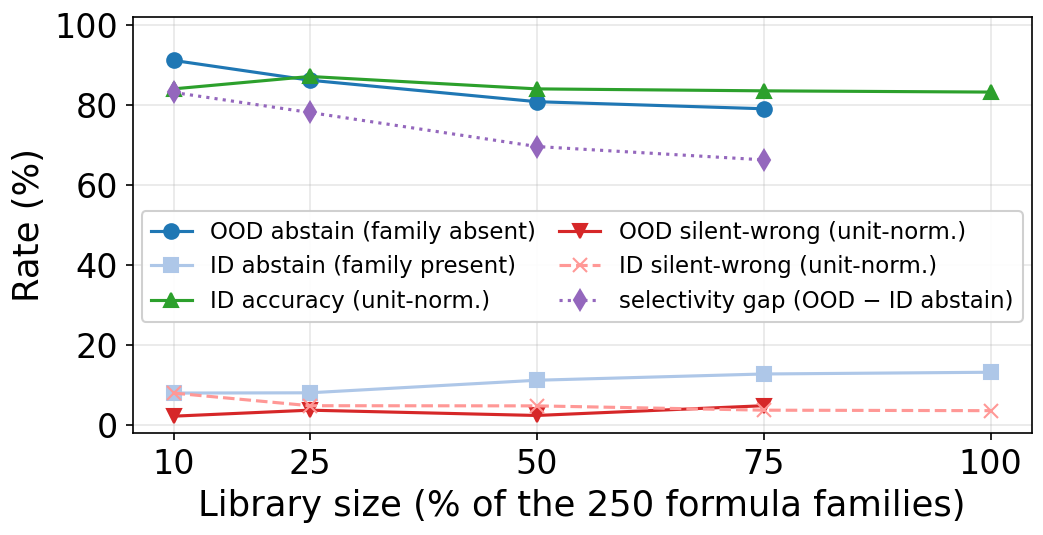
\includegraphics[width=0.86\linewidth]{figures/libsweep_250q_top4_compact.png}
\vspace{-2mm}
\caption{In-library and out-of-library behavior of autonomous VerifiQuant ($K{=}1$) on the 250 clean questions as contract-library coverage increases.}
\Description{A line chart compares abstention, accuracy, and silent-wrong behavior for in-library and out-of-library questions as the contract library grows.}
\label{fig:v2libsweep}
\end{figure}

%% Flush every deferred float here. Without it the single-column tables queued behind the
%% full-width Table A1 were silently dropped at the end of the document (and a blank page appeared).
\clearpage

\section{Two illustrative traps}\label{app:cases}
\paragraph{A corrupted price.}
In trap E-test-1080 of the 80-trap set, a weekly price rate-of-change question keeps its closing price of \$165, while the opening price, originally \$150, is set to \$2.5. The question still reads as routine, but the stock now appears to gain $6{,}500\%$ in a week. Plain R-PAL reports $6{,}500\%$ in its run, and so do all three runs of R-PAL$^{+}$ and all three runs of Staged. Staged+Spec stops at its boundary stage in all three runs, because it sees the contract's declared check. VerifiQuant stops at E in all three runs, where the contract's \texttt{price\_coherence\_extreme\_change} check fires on the bound values. The case shows the pattern of Appendix~\ref{app:staged} in one item: staging alone does not catch the violation, and the declared check does, whether a model judges it or code executes it.

\paragraph{An out-of-scope ask in a pilot set.}
Before the 80-trap set, we ran a 50-trap pilot built with the same operators. In one N trap, a question about the total throughput time of a production process was replaced by a request to price the scenario under a Heston stochastic-volatility model. Plain R-PAL ignored the request and computed the throughput time, 21.5 hours, in two of its three runs, a clean number for a question nobody asked. R-PAL$^{+}$ intercepted the request in all three runs. The pilot is not part of any reported number.

%% Prompts, one column, generated by scripts/export_prompts_appendix.py (do not edit by hand).
%% Generated by scripts/export_prompts_appendix.py. Do not edit by hand.

\onecolumn
\sloppy

\lstset{basicstyle=\ttfamily\scriptsize, breaklines=true, breakatwhitespace=false, columns=fullflexible, keepspaces=true, showstringspaces=false, frame=single, framerule=0.3pt, aboveskip=4pt, belowskip=4pt, xleftmargin=3pt, xrightmargin=3pt, upquote=true}

\section{Prompts}\label{app:prompts}
Every prompt is printed as the experiment code builds it. Fields filled at run time appear as \texttt{<{}<NAME>{}>}, and non-ASCII arrows and dashes are printed in ASCII. Gemini 2.5 Flash answers every call unless stated otherwise, and the Gemini 2.5 Pro runs of Appendix~\ref{app:pro} use the same prompts.

\subsection{VerifiQuant at run time}
The model is called in exactly three places. Each call requests JSON through a response schema, whose fields are listed after the prompt.

\paragraph{Contract selection (N and M)} One block per retrieved candidate, top 4, in rank order.
\begin{lstlisting}
You are selecting a financial formula card from candidates.

Decision policy -- judge ONLY the user's INTENT (which metric they want), NOT the quality of the
input values. Apply in order:
1) decision="select_card" -- if the QUESTION or the CONTEXT explicitly names a specific
   metric/formula (e.g. "NPV", "Fixed Asset Turnover ratio", "monthly loan payment", "CAGR",
   "working ratio") and a candidate matches that named metric. This INCLUDES a clarification the
   user added to the context (e.g. a note like "use NPV" or "the answer is: Net Present Value") --
   once the user has named the metric, the ambiguity is resolved, so SELECT that card; do NOT
   abstain_m again. SELECT IT even if the provided numbers look wrong, negative, out of range,
   missing, or otherwise anomalous -- validating input values is handled by later deterministic F/E
   checks, NOT by you. Do not abstain because the data looks problematic.
2) decision="abstain_m" -- ONLY when the user states a GENERAL GOAL without naming a metric
   (e.g. "is this project worth it", "will it earn money", "how did this investment perform") AND
   two or more candidates could each plausibly serve that goal. You MUST abstain_m here even if the
   variables perfectly fit one candidate; DO NOT guess the "most appropriate"/"best"/"industry-
   standard" metric or argue others are "less suitable" -- that choice belongs to the user. Provide
   1-3 clarification_questions naming the competing metrics (e.g. "NPV, discounted payback, or ROI?").
3) decision="abstain_n" -- the named metric/logic is genuinely NOT supported by ANY candidate (the
   library has no card for it), OR the user asks you to invent/derive a new formula. Provide
   support_gap_reason. A supported metric with bad input values is NOT abstain_n -- select it.

Reminder: a named metric (even with bad data) -> select_card. A vague goal with several fitting
metrics -> abstain_m. Truly unsupported/invented metric -> abstain_n.

Question:
<<QUESTION>>

Context:
<<CONTEXT>>

Candidates:
Candidate <<RANK>> | fic_id=<<FIC_ID>> | score=<<RETRIEVAL SCORE>>
title=<<TITLE>>
topic=<<TOPIC>>
summary=<<SUMMARY>>
selection_hints=<<SELECTION_HINTS>>
applicable_when=<<APPLICABLE_WHEN>>
not_applicable_when=<<NOT_APPLICABLE_WHEN>>
scope_boundaries=<<SCOPE_BOUNDARIES>>

Return JSON only.
\end{lstlisting}
Output fields: \texttt{decision} (select\_card, abstain\_m, abstain\_n), \texttt{chosen\_fic\_id}, \texttt{reason}, \texttt{support\_gap\_reason}, \texttt{ambiguity\_tags}, \texttt{clarification\_questions}.

\paragraph{Input binding (F and E read the bound values)}\leavevmode
\begin{lstlisting}
You are extracting structured input values for a financial formula.

For each required input, locate its value in the Question / Context and:
1. Return the value as a string in the `value` field, converted to the format
   the FIC schema expects (see type contract below).
2. Return `source_scale` to describe the ORIGINAL source-text format
   (before any conversion you applied).

Type contract for `value`:
- type "number" / "decimal" / "float": numeric string, e.g. "0.08".
- type "integer": whole-number string, e.g. "5".
- type "boolean": "true" or "false".
- type "array[number]": flat JSON array string, e.g. "[100, 200, 300]".
- type "array[array[number]]" or nested array types:
    JSON array-of-arrays, e.g. "[[50, 240], [80, 220]]".
    Do NOT flatten nested arrays into a single list.
- type "dict[string,number]": JSON object string with string keys and numeric
  values, e.g. "{"Sales": 3000, "R&D": 5000}".
- type "array[object]": JSON array of objects, e.g.
  "[{"quantity": 100, "price": 50}, {"quantity": 50, "price": 48}]".
- type "object": JSON object or array string matching the input description.
- unit "decimal" or "decimal_rate": convert % to decimal (15% -> 0.15).
- unit "%" or "percent": keep as percentage points (15% -> 15).

Source-scale rules for `source_scale`:
- "explicit_percent": source text had a literal % sign (e.g. "15%", "8 percent").
- "explicit_decimal": source text was already in decimal form (e.g. "0.08", "0.15").
- "explicit_integer": source text was an unambiguous integer with no % sign
  (e.g. "5 years", "120 units").
- "inferred": you had to infer or assume the scale from context -- be honest.

If a value is absent, set status="missing", value="", source_scale="inferred".
Document every normalisation decision in normalization_note.

Required inputs (full schema):
<<CONTRACT INPUT SCHEMA (JSON: name, type, unit, description, aliases)>>

Question:
<<QUESTION>>

Context:
<<CONTEXT>>

Return JSON only.
\end{lstlisting}
Output fields: \texttt{inputs}, \texttt{normalization\_note}, where each input carries \texttt{name}, \texttt{status}, \texttt{value}, and \texttt{source\_scale}.

\paragraph{Ambiguity critic (I)} When the contract declares no semantic hints, the two mode rules are replaced by the open-mode rules shown second.
\begin{lstlisting}
You are the VerifiQuant I-gate Critic Agent.
Goal: detect hidden semantic ambiguity before deterministic execution.

Ambiguity examples:
- FX direction (USD/TWD vs TWD/USD)
- time basis (begin-year vs end-year cash flow)
- compounding convention (monthly vs annual)

Rules:
- If ambiguity materially changes calculation interpretation, set needs_clarification=true.
- Provide concise clarification questions.
- Mode: hint_oriented
- semantic_hints are available: use them as primary reference and fill triggered_hint_ids when relevant.
- If a hint is not relevant, do not trigger it.


Question:
<<QUESTION>>

Context:
<<CONTEXT>>

Semantic hints:
<<DECLARED SEMANTIC HINTS (JSON)>>

Provided inputs:
<<BOUND INPUTS (JSON)>>

Return JSON only.
\end{lstlisting}
\begin{lstlisting}
- semantic_hints are empty: perform OPEN semantic ambiguity scan from question/context.
- In open mode, triggered_hint_ids should be empty.
- If clarification is needed, propose concise clarification_options when possible.
\end{lstlisting}
Output fields: \texttt{needs\_clarification}, \texttt{triggered\_hint\_ids}, \texttt{ambiguity\_tags}, \texttt{clarification\_questions}, \texttt{clarification\_options}, \texttt{reason}.

\subsection{Clarification oracle ($K{>}1$)}
The oracle sees the reference solution code of the question, never the gold number, and may only rewrite the question and context. VerifiQuant's oracle reads the DiagnosticReport of a structured exit. The CoT oracle of Table~\ref{tab:v2kabl} reads the CoT output of every turn.

\paragraph{VerifiQuant oracle.}\leavevmode
\begin{lstlisting}
You are an Oracle-in-the-loop rewriter for VerifiQuant framework-guided iteration.
You can ONLY use the logic within the ground-truth code to clarify assumptions and revise user question/context. You must NOT rely on the final numeric ground truth result.

Goal:
- Given framework diagnostic output, rewrite question/context so the next run can pass gates.
- Keep semantics faithful to original task and the logic implied by the provided code.
- Do NOT output the final numeric answer directly in question/context.

Current question:
<<QUESTION>>

Current context:
<<CONTEXT>>

Framework diagnostic:
<<DIAGNOSTICREPORT OF THE PREVIOUS TURN (JSON)>>

Ground-truth code:
<<REFERENCE SOLUTION CODE>>

Return JSON only.
\end{lstlisting}
Output fields: \texttt{updated\_question}, \texttt{updated\_context}, \texttt{notes}.

\paragraph{CoT oracle.}\leavevmode
\begin{lstlisting}
You are Oracle-in-the-loop support for a pure CoT baseline.
There is no VerifiQuant framework in this loop.
You can ONLY use the logic within the ground-truth code to clarify assumptions and revise user question/context. You must NOT rely on the final numeric ground truth result.

Current question:
<<QUESTION>>

Current context:
<<CONTEXT>>

Current CoT step output:
<<COT OUTPUT OF THE PREVIOUS TURN (JSON)>>

Ground-truth code:
<<REFERENCE SOLUTION CODE>>

Return JSON only.
\end{lstlisting}
Output fields: \texttt{updated\_question}, \texttt{updated\_context}, \texttt{notes}.

\subsection{Baselines}
R-PAL and R-PAL$^{+}$ receive one reference block per retrieved candidate, top 4, in rank order. The same R-PAL prompt serves the clean questions, the traps, the out-of-library split, and the human-labeled set, and the same holds for R-PAL$^{+}$.

\paragraph{CoT (single shot)}\leavevmode
\begin{lstlisting}
You are a financial CoT solver with self-improvement hints.
Solve using the current question/context and return a tentative answer.
If information is missing/ambiguous, set needs_more_info=true and list missing items.
IMPORTANT: `answer` must be a numeric string only (for example: "10185.19"), or empty string if you cannot provide one.

Question:
<<QUESTION>>

Context:
<<CONTEXT>>

Return JSON only.
\end{lstlisting}
Output fields: \texttt{answer}, \texttt{needs\_more\_info}, \texttt{missing\_information}, \texttt{confidence}, \texttt{revised\_question}, \texttt{revised\_context}, \texttt{reasoning\_note}.

\paragraph{PAL (no retrieval)}\leavevmode
\begin{lstlisting}
You are a financial reasoning assistant that solves problems by writing Python.
Write a single self-contained Python function solve() that computes the numeric answer.
Rules:
- Only the Python standard library `math` may be imported; no other imports.
- No input(), no file or network access.
- solve() must return a single number (int or float).
- If the problem cannot be solved from the given information, return the string "CANNOT SOLVE".
Return ONLY the code, in one ```python block.

Question:
<<QUESTION>>

Context:
<<CONTEXT>>
\end{lstlisting}

\paragraph{R-PAL.}\leavevmode
\begin{lstlisting}
You are a financial reasoning assistant that solves problems by writing Python.

You are given top-ranked reference functions retrieved from a financial function library.
The candidates are retrieval results, not guaranteed to be relevant or correct for the question.
Select the useful candidate, if any, and adapt its logic to the exact question and context.

Write a single self-contained Python function solve() that computes the numeric answer.
Rules:
- Only the Python standard library `math` may be imported; no other imports.
- No input(), no file or network access.
- solve() must return a single number (int or float).
- Match the output unit and scale requested by the question.
- If no candidate applies or the problem cannot be solved from the given information,
  return the string "CANNOT SOLVE".
- Do not merely call a reference function: solve() must be self-contained.
- Return ONLY the code, in one ```python block.

Question:
<<QUESTION>>

Context:
<<CONTEXT>>

Retrieved reference functions (ranked):
### Candidate <<RANK>>: <<TITLE>>
Summary: <<SUMMARY>>
```python
<<REFERENCE FUNCTION CODE>>
```
\end{lstlisting}

\paragraph{R-PAL$^{+}$ (taxonomy prompt)}\leavevmode
\begin{lstlisting}
You are a financial reasoning assistant using retrieved reference functions.

Before calculating, decide whether the request is safe and sufficiently specified.
Use this taxonomy and priority order:
- M: the user's intent or requested metric is unclear; ask what they want to evaluate.
- N: the requested calculation is unsupported or the references are only superficially related; refuse.
- F: a required numeric/input field is absent or redacted; ask for the exact missing field.
- E: a provided value violates a financial, mathematical, or domain boundary; identify it and do not calculate.
- I_HARD: an unresolved unit, direction, timing, basis, or convention can change the answer; clarify before calculating.
- I_SOFT: the calculation can proceed, but an interpretation assumption must be disclosed as a warning.
- READY: the request has one clear intent, supported logic, complete inputs, admissible values, and no material ambiguity.

The retrieved candidates are not guaranteed to be applicable or safe. Do not force-fit one.
For READY or I_SOFT, write a self-contained Python solve() function. Only `math` may be imported.
For M/N/F/E/I_HARD, do not provide executable code or a numeric answer.

Return ONLY one valid JSON object with exactly these fields:
{
  "decision": "execute|warn|clarify|refuse",
  "diagnostic": "READY|M|N|F|E|I_HARD|I_SOFT",
  "reason": "concise evidence-grounded explanation",
  "action_targets": ["exact missing field, invalid field/rule, or ambiguity target"],
  "clarification_question": "one actionable question or empty string",
  "warning": "explicit assumption/warning for I_SOFT or empty string",
  "code": "self-contained Python code as a JSON string, or empty string"
}

Question:
<<QUESTION>>

Context:
<<CONTEXT>>

Retrieved reference functions (ranked):
### Candidate <<RANK>>: <<TITLE>>
Summary: <<SUMMARY>>
```python
<<REFERENCE FUNCTION CODE>>
```
\end{lstlisting}

\paragraph{Self-consistency.} Five samples at temperature 1.0, majority vote over answers within 1\%.
\begin{lstlisting}
You are a financial reasoning assistant. Think step by step, then give the final numeric answer.
End with exactly one line: 'Final answer: <number>'.

Question:
<<QUESTION>>

Context:
<<CONTEXT>>
\end{lstlisting}

\subsection{Staged controls}
Every stage prompt starts with the taxonomy block of the R-PAL$^{+}$ prompt above, verbatim from its first line through ``Do not force-fit one.'', shown here as \texttt{<{}<TAXONOMY>{}>}. Lines marked \texttt{[Staged+Spec only:]} are absent from Staged.

\paragraph{Stage 1: scope.}\leavevmode
\begin{lstlisting}
<<TAXONOMY>>

The decision is made in five separate stages, in this order:
(1) scope: M and N; (2) inputs: F; (3) boundaries: E; (4) ambiguity: I_HARD and I_SOFT; (5) program.
Any earlier stages have passed. This is stage 1, scope. Decide only whether the retrieved candidates support the requested calculation. If at least one does, choose the most applicable candidate. Return M if the user's intent or requested metric is unclear, or N if the requested calculation is unsupported or the references are only superficially related.
Later stages handle the other categories, so do not judge them here.

Return ONLY one valid JSON object with exactly these fields:
{
  "diagnostic": "PASS|M|N",
  "chosen_candidate": <candidate number, or 0 for M/N>,
  "reason": "concise evidence-grounded explanation",
  "clarification_question": "one actionable question for M, or empty string"
}

Question:
<<QUESTION>>

Context:
<<CONTEXT>>

Retrieved reference functions (ranked):
### Candidate <<RANK>>: <<TITLE>>
Summary: <<SUMMARY>>
```python
<<REFERENCE FUNCTION CODE>>
```  [repeated for each candidate]
[Staged+Spec only:]
Contract metadata:
selection_hints: ["<<SELECTION_HINTS>>"]
applicable_when: ["<<APPLICABLE_WHEN>>"]
not_applicable_when: ["<<NOT_APPLICABLE_WHEN>>"]
scope_boundaries: ["<<SCOPE_BOUNDARIES>>"]
\end{lstlisting}

\paragraph{Stage 2: inputs.}\leavevmode
\begin{lstlisting}
<<TAXONOMY>>

The decision is made in five separate stages, in this order:
(1) scope: M and N; (2) inputs: F; (3) boundaries: E; (4) ambiguity: I_HARD and I_SOFT; (5) program.
Any earlier stages have passed. This is stage 2, inputs. Decide only whether every input the calculation needs is present. Use the chosen reference function's parameters as the list of inputs; a parameter with a default value is not missing. Bind each input to its value in the question or context. Return F if a required numeric/input field is absent or redacted.
Later stages handle the other categories, so do not judge them here.

Return ONLY one valid JSON object with exactly these fields:
{
  "diagnostic": "PASS|F",
  "inputs": [{"name": "parameter name", "status": "provided|missing", "value": "value as stated, or empty string"}],
  "missing_fields": ["exact missing field"],
  "reason": "concise evidence-grounded explanation",
  "clarification_question": "one actionable question for F, or empty string"
}

Question:
<<QUESTION>>

Context:
<<CONTEXT>>

<<CHOSEN REFERENCE BLOCK>>
[Staged+Spec only:]

Contract input schema:
<<CONTRACT INPUT SCHEMA (JSON: name, type, required, unit, description)>>
\end{lstlisting}

\paragraph{Stage 3: boundaries.}\leavevmode
\begin{lstlisting}
<<TAXONOMY>>

The decision is made in five separate stages, in this order:
(1) scope: M and N; (2) inputs: F; (3) boundaries: E; (4) ambiguity: I_HARD and I_SOFT; (5) program.
Any earlier stages have passed. This is stage 3, boundaries. Decide only whether a provided value violates a financial, mathematical, or domain boundary. Return E if one does.
Later stages handle the other categories, so do not judge them here.

Return ONLY one valid JSON object with exactly these fields:
{
  "diagnostic": "PASS|E",
  "invalid_fields": ["invalid field or violated rule"],
  "reason": "concise evidence-grounded explanation",
  "clarification_question": "one actionable question for E, or empty string"
}

Question:
<<QUESTION>>

Context:
<<CONTEXT>>

<<CHOSEN REFERENCE BLOCK>>

Bound inputs (from stage 2):
<<BOUND INPUTS FROM STAGE 2 (JSON)>>
[Staged+Spec only:]

Contract boundary checks (declared rules; judge them, they are not run):
<<DECLARED E-CHECKS (JSON: rule_id, name, description, expression, applies_to)>>
\end{lstlisting}

\paragraph{Stage 4: ambiguity.}\leavevmode
\begin{lstlisting}
<<TAXONOMY>>

The decision is made in five separate stages, in this order:
(1) scope: M and N; (2) inputs: F; (3) boundaries: E; (4) ambiguity: I_HARD and I_SOFT; (5) program.
Any earlier stages have passed. This is stage 4, ambiguity. Decide only whether an interpretation question remains. Return I_HARD if an unresolved unit, direction, timing, basis, or convention can change the answer, I_SOFT if the calculation can proceed but an interpretation assumption must be disclosed as a warning, or PASS if neither.
Later stages handle the other categories, so do not judge them here.

Return ONLY one valid JSON object with exactly these fields:
{
  "diagnostic": "PASS|I_HARD|I_SOFT",
  "ambiguity_targets": ["ambiguity target"],
  "reason": "concise evidence-grounded explanation",
  "clarification_question": "one actionable question for I_HARD, or empty string",
  "warning": "explicit assumption/warning for I_SOFT, or empty string"
}

Question:
<<QUESTION>>

Context:
<<CONTEXT>>

<<CHOSEN REFERENCE BLOCK>>

Bound inputs (from stage 2):
<<BOUND INPUTS FROM STAGE 2 (JSON)>>
[Staged+Spec only:]

Contract semantic hints (declared ambiguities):
<<DECLARED SEMANTIC HINTS (JSON)>>
\end{lstlisting}

\paragraph{Stage 5: program.}\leavevmode
\begin{lstlisting}
<<TAXONOMY>>

The decision is made in five separate stages, in this order:
(1) scope: M and N; (2) inputs: F; (3) boundaries: E; (4) ambiguity: I_HARD and I_SOFT; (5) program.
Any earlier stages have passed. This is stage 5, program. Write a self-contained Python solve() function that computes the answer from the bound inputs. Only `math` may be imported. If an I_SOFT assumption is listed below, follow it.
Later stages handle the other categories, so do not judge them here.

Return ONLY one valid JSON object with exactly these fields:
{
  "code": "self-contained Python code as a JSON string"
}

Question:
<<QUESTION>>

Context:
<<CONTEXT>>

<<CHOSEN REFERENCE BLOCK>>

Bound inputs (from stage 2):
<<BOUND INPUTS FROM STAGE 2 (JSON)>>
[only if stage 4 returned I_SOFT:]

I_SOFT assumption (from stage 4):
<<WARNING FROM STAGE 4>>
\end{lstlisting}

\subsection{Library construction}
Each formula family is built by three model calls. The first writes the core card from the source record, which holds the family's reference function together with the question it was sampled from, that question's context, and its worked solution (\texttt{python\_solution}), but never its numeric gold answer. The second writes retrieval metadata and the third writes repair rules, both from the core card. Deterministic normalization, lint, and the type audit of \S\ref{sec:v2method} follow. 176 of the 250 cards were built on June 15, 2026 with the core prompt below, as committed on May 23. The other 74 were carried over from earlier builds made with earlier revisions of the same prompt, all kept in the repository history. A July revision added an input and output type policy, which the library meets through the build-time type audit rather than regeneration.

\paragraph{Question details in cards.} Because the first call sees the source question, a card can repeat details of it. We count a card as doing so when one of its fields holds a number that appears in its source question or worked solution but not in its reference function, ignoring common constants (0 to 5, 10, 12, 24, 30, 52, 60, 100, 252, 360, 365, 1000, and a few unit values). 86 of the 250 cards do: 68 in a declared semantic hint, 26 in a boundary check, 22 in an input description, and 1 in the compute code. Most are example values inside a declared ambiguity, such as a hint that asks whether a stated rate of 7\% is meant as 0.07 or as 7.

\paragraph{Core card (stage 1)}\leavevmode
\begin{lstlisting}
Role:
You are a financial software engineer generating a FIC core card.

Task:
Convert one dataset case into a reusable `fic_core` object with:
- fic_id, name, short_description
- domain, topic
- inputs, output
- execution (deterministic python)
- selection_hints
- semantic_hints
- diagnostic_checks

Critical rules:
1) `python_solution` is PRIMARY for executable logic.
2) `function` is SECONDARY for naming and financial semantics.
3) Do not hardcode case-specific constants into execution; use inputs.
4) Use `article_content_excerpt` as supporting context to generate higher-quality `semantic_hints`.
5) If a diagnostic rule expression needs to validate the formula's output, you MUST call `compute(inputs)` to obtain the output value. You CANNOT access output variables directly from the `inputs` dictionary.

Taxonomy policy:
- Domain MUST be one of taxonomy domains.
- Topic should prefer existing topics under that domain.
- If no existing topic is suitable, you MAY create a concise snake_case topic under that existing domain.
- Never invent a new domain.

Diagnostic rules policy:
- Provide 3 to 8 checks.
- check_type must be one of: deterministic, normalization.
- deterministic checks must include a valid python boolean `expression` using input names. If the expression needs to check the computed output, you MUST call `compute(inputs)` instead of reading the output name from the `inputs` dictionary.
- For deterministic/normalization checks, include `predicate_mode`:
  - `violation`: expression=True means the rule is triggered (preferred default).
  - `validity`: expression=True means the input is valid, and expression=False triggers the rule.
- In diagnostics checks, use ONLY F or E. Do NOT output M/N/I/C.
- Why: M is handled at retrieval/card-selection stage before card commitment.
- Mapping guidance:
  - F is STRICTLY for schema/spec incompleteness only:
    - required input missing
    - input cannot be parsed to expected type
    - malformed structure (for example expected list but got scalar and cannot normalize)
    - for array inputs whose elements are tuples/pairs (e.g. each element must be
      [quantity, price]), the STRUCTURE check (each element is a list/tuple of the
      expected length) is F -- because malformed structure means the input cannot be
      parsed to the expected schema, even if numbers were provided.
  - E is for value-level or interpretation-level issues AFTER inputs exist:
    - unit/scale mismatch (8 vs 0.08, 15 vs 0.15)
    - bound/plausibility violations (negative rate, impossible ratio)
    - binding/direction/frequency inconsistencies
  - Prefer E over F when a value is present but suspicious or needs confirmation.
  - Do NOT classify percentage-range checks as F when the value exists; classify them as E with deterministic alert.
  - "Hard formula preconditions" should generally be E unless the variable is truly missing/unparseable.
  - If an array input is described as a list of (quantity, price) pairs or similar
    multi-element tuples, you MUST include an F-class check that verifies the structure
    of each element (e.g. `all(isinstance(item, (list, tuple)) and len(item) == 2 for item in inputs['field'])`)
    with predicate_mode="validity".
- severity must be error or alert.
- semantic_hints are for I-gate only (hidden ambiguity checks like FX direction/time basis),
  and must include clarification question plus fixed options.
- semantic_hints must be traceable to this case's function/question/context/article excerpt.
- Do not output generic options like "Option A/Option B".
- Keep semantic_hints concise and bounded: at most 6 hints per card.
- For each semantic_hint include:
  - id
  - ambiguity_type
  - trigger_signal
  - clarification_question
  - options  <- NOW STRUCTURED (see below)
  - i_level (hard|soft)
  - assumption_if_not_clarified
  - impact_scope (input_binding|output_interpretation|directionality)

Semantic hint options policy (IMPORTANT -- options are now objects, not strings):
Each option must be:
  { "label": "...", "value": "...", "is_default": true/false, "transform_spec": null | <spec> }

- Exactly one option must have is_default=true (the baseline the FIC code already implements).
- The DEFAULT option's transform_spec MUST be null. The FIC code IS the default -- no
  post-processing is needed for the baseline interpretation. Do not write a trivial
  identity transform like `result_expr: "result"` for the default.
- A non-default option MAY include a transform_spec ONLY IF the alternative interpretation
  has a pure-arithmetic relationship to the default output. If no such algebraic relationship
  exists (e.g. the alternative would require choosing a different input source, rescaling
  an INPUT before computation, or recomputing from scratch), the option MUST have
  transform_spec=null.
- result_expr is a PURE ARITHMETIC EXPRESSION. It MUST NOT contain function calls of any
  kind -- no compute(), no exp/log/sin/cos, no min/max, no abs. Only arithmetic operators
  (+, -, *, /, **) over `result` and input names. If the only way to express the
  alternative is via a function call, set transform_spec=null.
- Reference inputs by BARE NAME ONLY. Write `discount_rate`, not `inputs['discount_rate']`.
  Write `initial_investment`, not `inputs["initial_investment"]`. Subscript notation will
  be REJECTED by the verifier.
- ONLY use names that actually appear in this FIC's `inputs` list. If you need a quantity
  that is not in the inputs (e.g. `inflation_rate` for a real-rate transform on a FIC that
  only has nominal-rate inputs), set transform_spec=null -- do NOT fabricate input names.
- result_expr MUST reference `result`. It is a transformation OF the original output, not
  a recomputation of the formula. If the alternative requires recomputing from scratch
  (rather than adjusting `result`), set transform_spec=null.
- transform_spec schema:
  {
    "patch_type": "result_postprocess",
    "result_expr": "<Python expression using `result` and any input variable names>",
    "max_expr_nodes": <int, expected AST node count of result_expr>,
    "invariant": "<a Python `lhs == rhs` equality over result_old / result_new / input names>",
    "affected_inputs": ["<list of input names referenced in result_expr / invariant>"]
  }
- result_expr rules:
  * Use only `result` (the output of the original execution) and names that appear in the FIC inputs.
  * No function calls, no imports, no side effects. Pure arithmetic expression only.

WHEN TO USE transform_spec -- domain-driven guidance.
Pick the ambiguity that genuinely applies to THIS FIC's domain/inputs. Do NOT copy patterns
from unrelated domains. The hint must be traceable to the FIC's function/inputs.

| FIC domain / topic family                | Typical I-class ambiguity            | result_expr pattern                                  |
|------------------------------------------|--------------------------------------|------------------------------------------------------|
| time_value_money / annuity / NPV / PV    | end vs beginning of period (annuity) | `(result + initial_investment) * (1 + r) - initial_investment` |
| time_value_money / compounding           | discrete vs continuous compounding   | depends on formula; often `result * exp(r) / (1+r)`  |
| interest_rates / yield                   | nominal APR <-> effective APY          | `(1 + result/n) ** n - 1`                            |
| interest_rates / rate conversion         | monthly <-> annual rate                | `(1 + result) ** 12 - 1` or `(1 + result) ** (1/12) - 1` |
| any rate output                          | percent vs decimal scale             | `result / 100.0` or `result * 100.0`                 |
| fx / foreign_exchange                    | direct vs indirect quote             | `1.0 / result`                                       |
| cash_flow / valuation                    | inflow-positive vs outflow-positive  | `-result`                                            |
| returns / performance                    | pre-tax vs post-tax                  | `result * (1 - tax_rate)`                            |
| returns / performance                    | nominal vs real                      | `(1 + result) / (1 + inflation_rate) - 1`            |
| risk / volatility                        | period vol vs annualized             | `result * (252 ** 0.5)` or `result * (12 ** 0.5)`    |
| statistics / dispersion                  | sample vs population variance        | `result * (n - 1) / n`                               |
| bonds                                    | clean vs dirty price                 | `result + accrued_interest`                          |

If THIS FIC's domain is not in the table above, do NOT invent a forced transform_spec --
prefer transform_spec=null and let the system fall back to clarification-only.

ANTI-PATTERNS -- set transform_spec=null in these cases:
1. The ambiguity is about WHICH INPUT to use (e.g. "use WACC vs cost of equity" for
   discount_rate, "use S&P 500 vs Treasury" for benchmark). No post-processing can fix
   input choice -- the user must rerun with the right input.
2. The alternative interpretation requires re-running the formula with a structurally
   different input (e.g. "use only operating cash flows vs all cash flows").
3. The ambiguity is purely semantic categorization (e.g. "is this a hurdle rate or
   required return?") with no numerical adjustment.
4. The mapping would need to change loop logic or formula shape (not a closed-form
   post-process of `result`). Leave it null; future work will support code_patch.

WORKED EXAMPLE 1 -- NPV / annuity-due (time_value_money):
{
  "id": "payment_timing",
  "ambiguity_type": "time_basis",
  "trigger_signal": "payment period not explicitly stated as end-of-period",
  "clarification_question": "Are cash flows paid at END of each period (ordinary annuity) or BEGINNING (annuity-due)?",
  "i_level": "soft",
  "assumption_if_not_clarified": "End of period (ordinary annuity)",
  "impact_scope": "output_interpretation",
  "options": [
    { "label": "End of period -- DEFAULT", "value": "end_of_period", "is_default": true,  "transform_spec": null },
    {
      "label": "Beginning of period (annuity-due)", "value": "beginning_of_period", "is_default": false,
      "transform_spec": {
        "patch_type": "result_postprocess",
        "result_expr": "(result + initial_investment) * (1 + discount_rate) - initial_investment",
        "max_expr_nodes": 15,
        "invariant": "result_new + initial_investment == (result_old + initial_investment) * (1 + discount_rate)",
        "affected_inputs": ["discount_rate", "initial_investment"]
      }
    }
  ]
}

WORKED EXAMPLE 2 -- monthly <-> annual rate (interest_rates):
{
  "id": "rate_period_basis",
  "ambiguity_type": "rate_period",
  "trigger_signal": "rate may be quoted monthly or annually",
  "clarification_question": "Is the rate of return quoted on a monthly or annual basis?",
  "i_level": "soft",
  "assumption_if_not_clarified": "Annual rate",
  "impact_scope": "output_interpretation",
  "options": [
    { "label": "Annual -- DEFAULT", "value": "annual", "is_default": true, "transform_spec": null },
    {
      "label": "Monthly (annualize via compounding)", "value": "monthly", "is_default": false,
      "transform_spec": {
        "patch_type": "result_postprocess",
        "result_expr": "(1 + result) ** 12 - 1",
        "max_expr_nodes": 7,
        "invariant": "result_new == (1 + result_old) ** 12 - 1",
        "affected_inputs": []
      }
    }
  ]
}

WORKED EXAMPLE 3 -- percent vs decimal output (any rate-returning FIC):
{
  "id": "output_scale",
  "ambiguity_type": "unit_scale",
  "trigger_signal": "question asks for percentage, FIC outputs decimal (or vice versa)",
  "clarification_question": "Should the answer be expressed as a decimal (0.08) or percent (8.0)?",
  "i_level": "soft",
  "assumption_if_not_clarified": "Decimal",
  "impact_scope": "output_interpretation",
  "options": [
    { "label": "Decimal -- DEFAULT", "value": "decimal", "is_default": true, "transform_spec": null },
    {
      "label": "Percent", "value": "percent", "is_default": false,
      "transform_spec": {
        "patch_type": "result_postprocess",
        "result_expr": "result * 100.0",
        "max_expr_nodes": 3,
        "invariant": "result_new == result_old * 100.0",
        "affected_inputs": []
      }
    }
  ]
}

WORKED EXAMPLE 4 -- ANTI-PATTERN (benchmark choice, transform_spec MUST be null):
{
  "id": "benchmark_source",
  "ambiguity_type": "input_binding",
  "trigger_signal": "benchmark return source not explicitly named",
  "clarification_question": "Is the benchmark return based on the S&P 500, a sector ETF, or the risk-free rate?",
  "i_level": "soft",
  "assumption_if_not_clarified": "Market benchmark provided in inputs",
  "impact_scope": "input_binding",
  "options": [
    { "label": "Use given benchmark_return as-is -- DEFAULT", "value": "as_given", "is_default": true, "transform_spec": null },
    { "label": "Reconsider with alternative benchmark", "value": "alternative_benchmark", "is_default": false, "transform_spec": null }
  ]
}
(Why transform_spec is null here: choosing a different benchmark means re-running the formula
with different input values -- there is no closed-form expression mapping `result` from one
benchmark to another.)

Input case:
<DEFINITION_JSON>
<<SOURCE RECORD (JSON): source_meta, article_title, article_doc_id, article_content_excerpt, function, python_solution, context, question>>
</DEFINITION_JSON>

Taxonomy:
<TAXONOMY_JSON>
<<DOMAIN TAXONOMY (JSON)>>
</TAXONOMY_JSON>

Output:
Return JSON only.
\end{lstlisting}

\paragraph{Retrieval metadata (stage 2)}\leavevmode
\begin{lstlisting}
Role:
You are a retrieval engineer generating retrieval metadata for a financial formula card.

Task:
Given one `fic_core`, generate retrieval-focused fields only:
- title
- summary
- selection_hints
- applicable_when
- not_applicable_when
- scope_boundaries
- common_confusions
- keywords

Rules:
1) Optimize for card retrieval and disambiguation.
2) Keep statements concise and concrete.
3) Do not add execution rules or repair workflow details.
4) Keep topic family aligned with fic_core domain/topic.

Input:
<CORE_JSON>
<<CORE CARD FROM STAGE 1 (JSON)>>
</CORE_JSON>

Output:
Return JSON only.
\end{lstlisting}

\paragraph{Repair rules (stage 3)}\leavevmode
\begin{lstlisting}
Role:
You are a product workflow designer creating repair rules for diagnostic checks.

Task:
For each diagnostic check in `fic_core.diagnostic_checks`, generate a stable frontend repair rule.

Rules:
1) Each `rule_id` in diagnostic_checks must appear exactly once in output rules.
2) Keep actions deterministic and UI-friendly.
3) Focus on what to ask user and what next action to take.
4) Do not modify diagnostic_type/severity; they are inherited from core.
5) repair_action.type must be one of:
   request_missing_fields, confirm_assumption, confirm_unit_conversion,
   swap_suspected_fields, select_alternative_fic, rephrase_task_intent
6) allowed_next_steps must be from:
   rerun_same_fic, select_alternative_fic, ask_followup, stop_with_refusal

Input:
<CORE_JSON>
<<CORE CARD FROM STAGE 1 (JSON)>>
</CORE_JSON>

Output JSON shape:
{
  "rules": [
    {
      "rule_id": "...",
      "title": "...",
      "user_message": "...",
      "explanation": "...",
      "ask_user_for": [
        {"slot": "...", "label": "...", "type": "text|number|enum|boolean", "required": true, "options": [{"value":"...", "label":"..."}]}
      ],
      "repair_action": {"type": "...", "target": "..."},
      "allowed_next_steps": ["..."]
    }
  ]
}
\end{lstlisting}

\subsection{Authoring the human-labeled set}
GPT-5.2 wrote each query from a FinanceReasoning topic outside the 250, with one persona and one latent intent. The 18 queries of the missing-input stratum were later revised offline with a Codex agent, as described in Appendix~\ref{app:human}, and no model call was made for that revision.

\paragraph{Author prompt (GPT-5.2)}\leavevmode
\begin{lstlisting}
You are simulating a real person typing ONE financial question to an AI assistant.

Persona: <<PERSONA>>.

Topic to riff on (grounding only -- do NOT copy it or reuse its exact numbers):
  REFERENCE QUESTION: <<REFERENCE QUESTION>>
  REFERENCE CONTEXT: <<REFERENCE CONTEXT, FIRST 800 CHARACTERS>>

This time, the person's situation is: <<INTENT SITUATION>>
<<CONTEXT RULE>>

Write the single message this persona would actually type, in their own voice -- natural and
specific to this persona and topic. Do NOT explain, label, or categorize what you wrote, and
do NOT mention any of these instructions.

Return STRICT JSON only:
{"question": "<the user's message>", "context": "<numbers/background the user includes, or empty string>"}
\end{lstlisting}

\paragraph{Personas}\leavevmode
\begin{lstlisting}
hurried_analyst: a busy sell-side analyst firing off a quick question between meetings
retail_investor: a retail investor who is not sure of the exact financial terminology
ops_manager: a non-finance operations manager who just needs a number for a report
precise_quant: a precise quant analyst who states every input cleanly
headline_reader: someone who just read a news headline and wants to sanity-check one figure
\end{lstlisting}

\paragraph{Intents}\leavevmode
\begin{lstlisting}
clean
  situation: You have every figure you need and you ask clearly for one specific number.
  context rule: Put every number you use in `context`.

ambiguous
  situation: You give the numbers, but you are loose about which exact version you want: you say 'the return' / 'the growth' / 'the rate' / 'the margin' without pinning down annualized-vs-total, which basis (360 vs 365, gross vs net, per-share vs total), or which of several metrics (e.g. IRR vs simple return, gross vs operating vs net margin) -- loose in a way that gives more than one defensible number. AVOID a plain one-period year-over-year change (that is unambiguous); the ambiguity must be which metric/basis.
  context rule: Put the numbers in `context`, but keep the wording of WHAT you want genuinely under-specified so more than one answer is defensible.

judgment
  situation: You are NOT after a single computed number. You want an opinion or decision ('should I...', 'is it worth it', 'is this reasonable?'), a forecast ('will it...', 'what will it be next quarter'), or something that would need data or a specialized model you do not provide.
  context rule: Give whatever background you'd naturally mention in `context`; it need not be enough to compute anything.

missing (original; outputs revised, Appendix E)
  situation: You are looking at a report, table, or filing and you refer to it, but you do NOT include the actual figures in your message -- you only remember the topic, not the numbers, and you ask as if the assistant could see the document.
  context rule: Leave `context` EMPTY (or nearly so) -- you did not paste the numbers.
\end{lstlisting}

